\documentclass[11pt]{article}
\usepackage[margin=1in]{geometry}
\usepackage{amsmath,amssymb}
\usepackage{graphicx}
\usepackage{hyperref}
\usepackage{booktabs}
\usepackage{enumitem}
\usepackage{caption}

\title{Ensemble-Based SIDM Weak-Lensing Forecasts for Spec-S5 White-Paper Use}
\author{}
\date{\today}

\begin{document}
\maketitle

\section{Executive Summary}

\subsection{Dwarf lenses}
Building on Yi-Fei Luo's single-halo SIDM forecasting baseline, we implement an ensemble-level forecast in which dwarf lenses are sampled as a stellar-mass-selected population and propagated through SHMR scatter, halo concentration scatter, profile projection, and stacked $\Delta\Sigma(R)$. The key result is methodological: the SIDM--CDM contrast is evaluated for a \emph{distribution} of halo properties rather than one fiducial halo, which is a better match to the stacked-lensing observable expected from Spec-S5 + Stage-IV imaging.

\subsection{Cluster lenses}
For clusters, we implement a halo-mass-selected ensemble forecast and include Tier-2 hybrid profile modeling (SIDM-modified inner halo plus DK14-like outer structure). This provides a realistic baseline for stacked $\Delta\Sigma$ comparisons, but the scientific interpretation remains systematics-limited: off-centering, concentration-population effects, and especially baryonic physics can generate profile changes that are degenerate with SIDM-induced modifications over overlapping radial ranges.

\section{Motivation and Scope}
The science goal is to test whether the expanded spectroscopic lens samples from Spec-S5, combined with Stage-IV weak lensing, can distinguish CDM from SIDM using stacked galaxy--galaxy lensing signals in dwarf and cluster regimes. The present implementation is intentionally a controlled first-order forecast:
\begin{itemize}[leftmargin=1.5em]
    \item no 2-halo term,
    \item no explicit off-centering model,
    \item no baryonic response model,
    \item no full survey covariance treatment.
\end{itemize}
These omissions are deliberate for transparency and speed; they define the caveats on absolute interpretability.

\section{Method Summary (Main Text)}
\subsection{Halo ensemble extension}
The primary contribution of this work is replacing a single-fiducial-halo calculation with a sampled halo ensemble:
\begin{itemize}[leftmargin=1.5em]
    \item \textbf{HMF mode (clusters):} sample from $dn/dM$ with selection and redshift distributions.
    \item \textbf{SHMR mode (dwarfs):} sample stellar masses, map to halo masses via SHMR with scatter, and apply concentration scatter.
\end{itemize}
Profiles are generated halo-by-halo, projected to $\Sigma(R)$ and $\Delta\Sigma(R)$, interpolated to common radial bins, and stacked.

\subsection{Profile model assumptions}
SIDM inner profiles are generated with the \texttt{parametricSIDM} wrapper. Tier-2 uses a DK14-like outer profile attachment and smooth stitching to avoid projection artifacts. In the checked-in default configs used for the summary figures, Tier-3 empirical outskirts correction is disabled.

\subsection{Projected lensing and toy distinguishability}
The local projection implementation computes
\begin{align}
\Sigma(R) &= 2\int_0^{z_{\max}}\rho\!\left(\sqrt{R^2+z^2}\right)\,dz,\\
\bar{\Sigma}(<R) &= \frac{2}{R^2}\int_0^R\Sigma(R')R'\,dR',\\
\Delta\Sigma(R) &= \bar{\Sigma}(<R)-\Sigma(R),
\end{align}
with log-space interpolation and stable numerical quadrature. Distinguishability is summarized with a toy
\begin{align}
\Delta\chi^2 = \sum_i \frac{\left[\Delta\Sigma_i^{\mathrm{SIDM}}-\Delta\Sigma_i^{\mathrm{CDM}}\right]^2}{\sigma_i^2},
\end{align}
using simple fractional-error scenarios.

\section{Representative Forecast Products}

\begin{figure}[htbp]
    \centering
    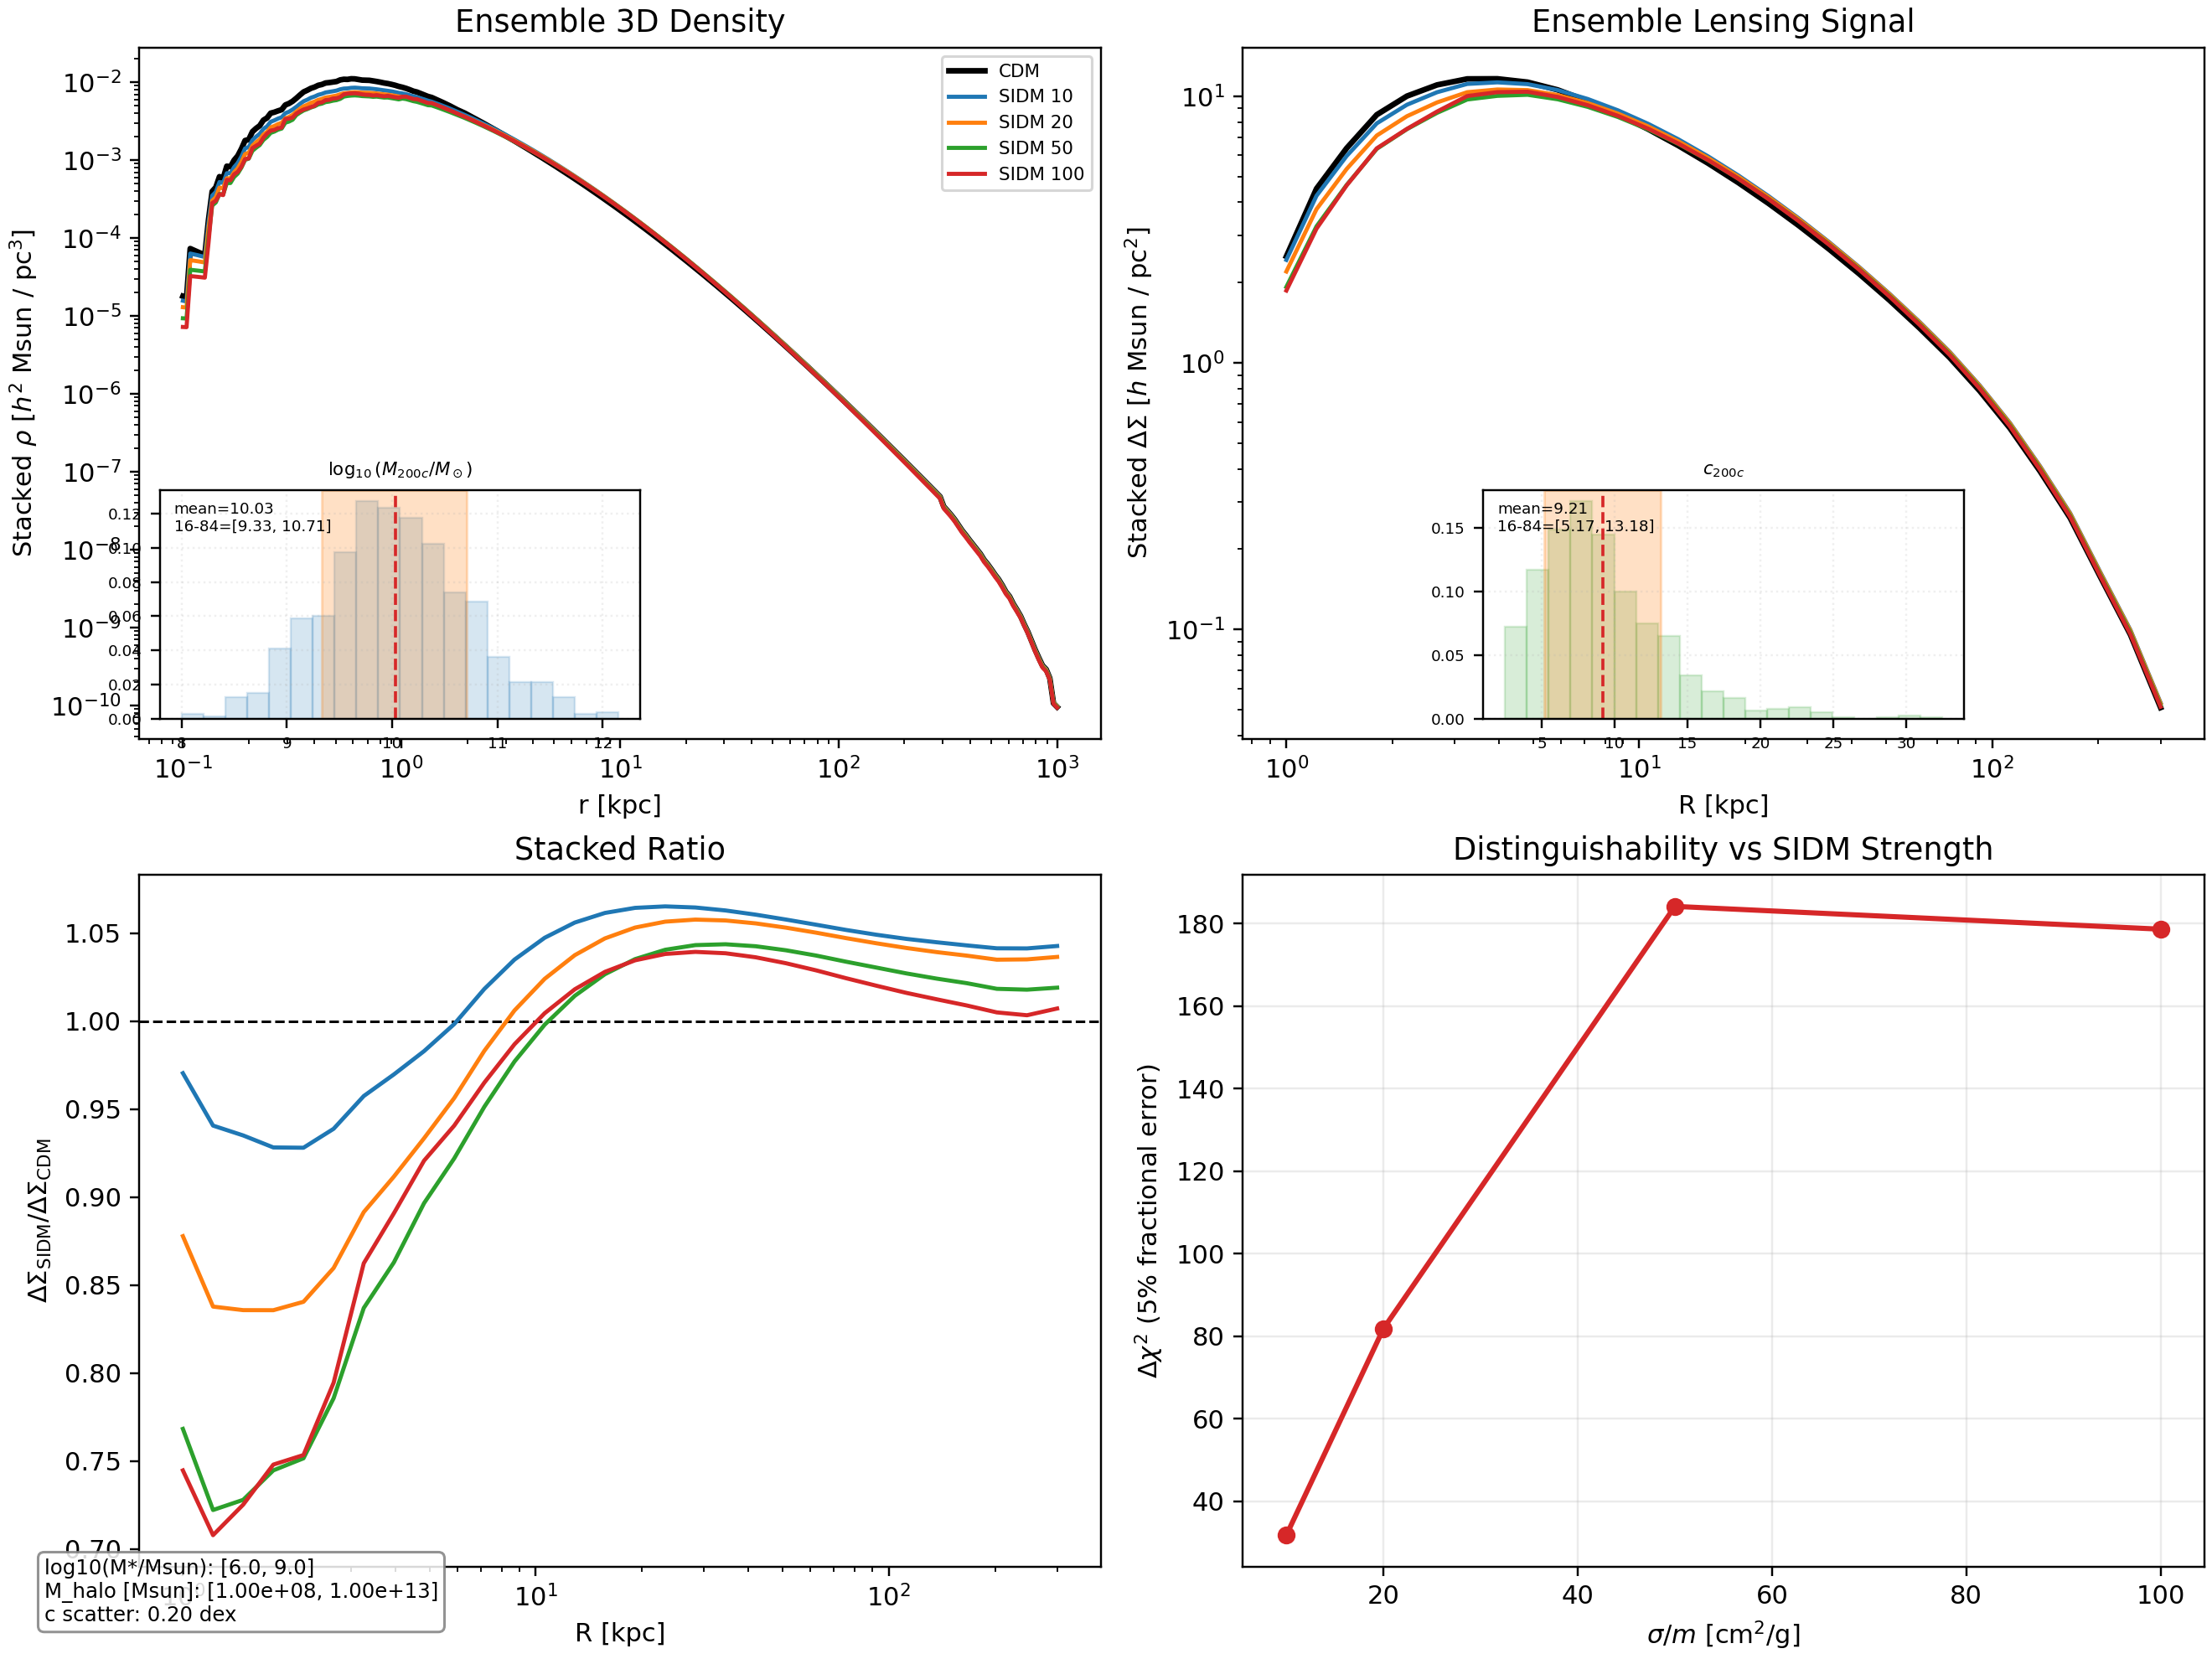
\includegraphics[width=0.92\textwidth]{figures/dwarf_ensemble_summary.png}
    \caption{\textbf{Dwarf ensemble summary (SHMR-selected sample).} Multi-panel diagnostic from the current default dwarf configuration (\texttt{docs/dwarf\_ensemble\_config.yaml}). The density panel and lensing panel show stacked CDM and SIDM predictions over the benchmark high-$\sigma/m$ grid; the ratio panel shows SIDM/CDM in projected space; the $\Delta\chi^2$ panel gives toy distinguishability under the assumed fractional-error model. Inset histograms report the sampled halo-mass and concentration distributions (including mean and 16--84\% ranges), making explicit that the forecast is population-based rather than single-halo. Units follow the project convention: stacked $\rho$ in $h^2\,M_\odot\,\mathrm{pc}^{-3}$ and stacked $\Delta\Sigma$ in $h\,M_\odot\,\mathrm{pc}^{-2}$.}
    \label{fig:dwarf_summary}
\end{figure}

\begin{figure}[htbp]
    \centering
    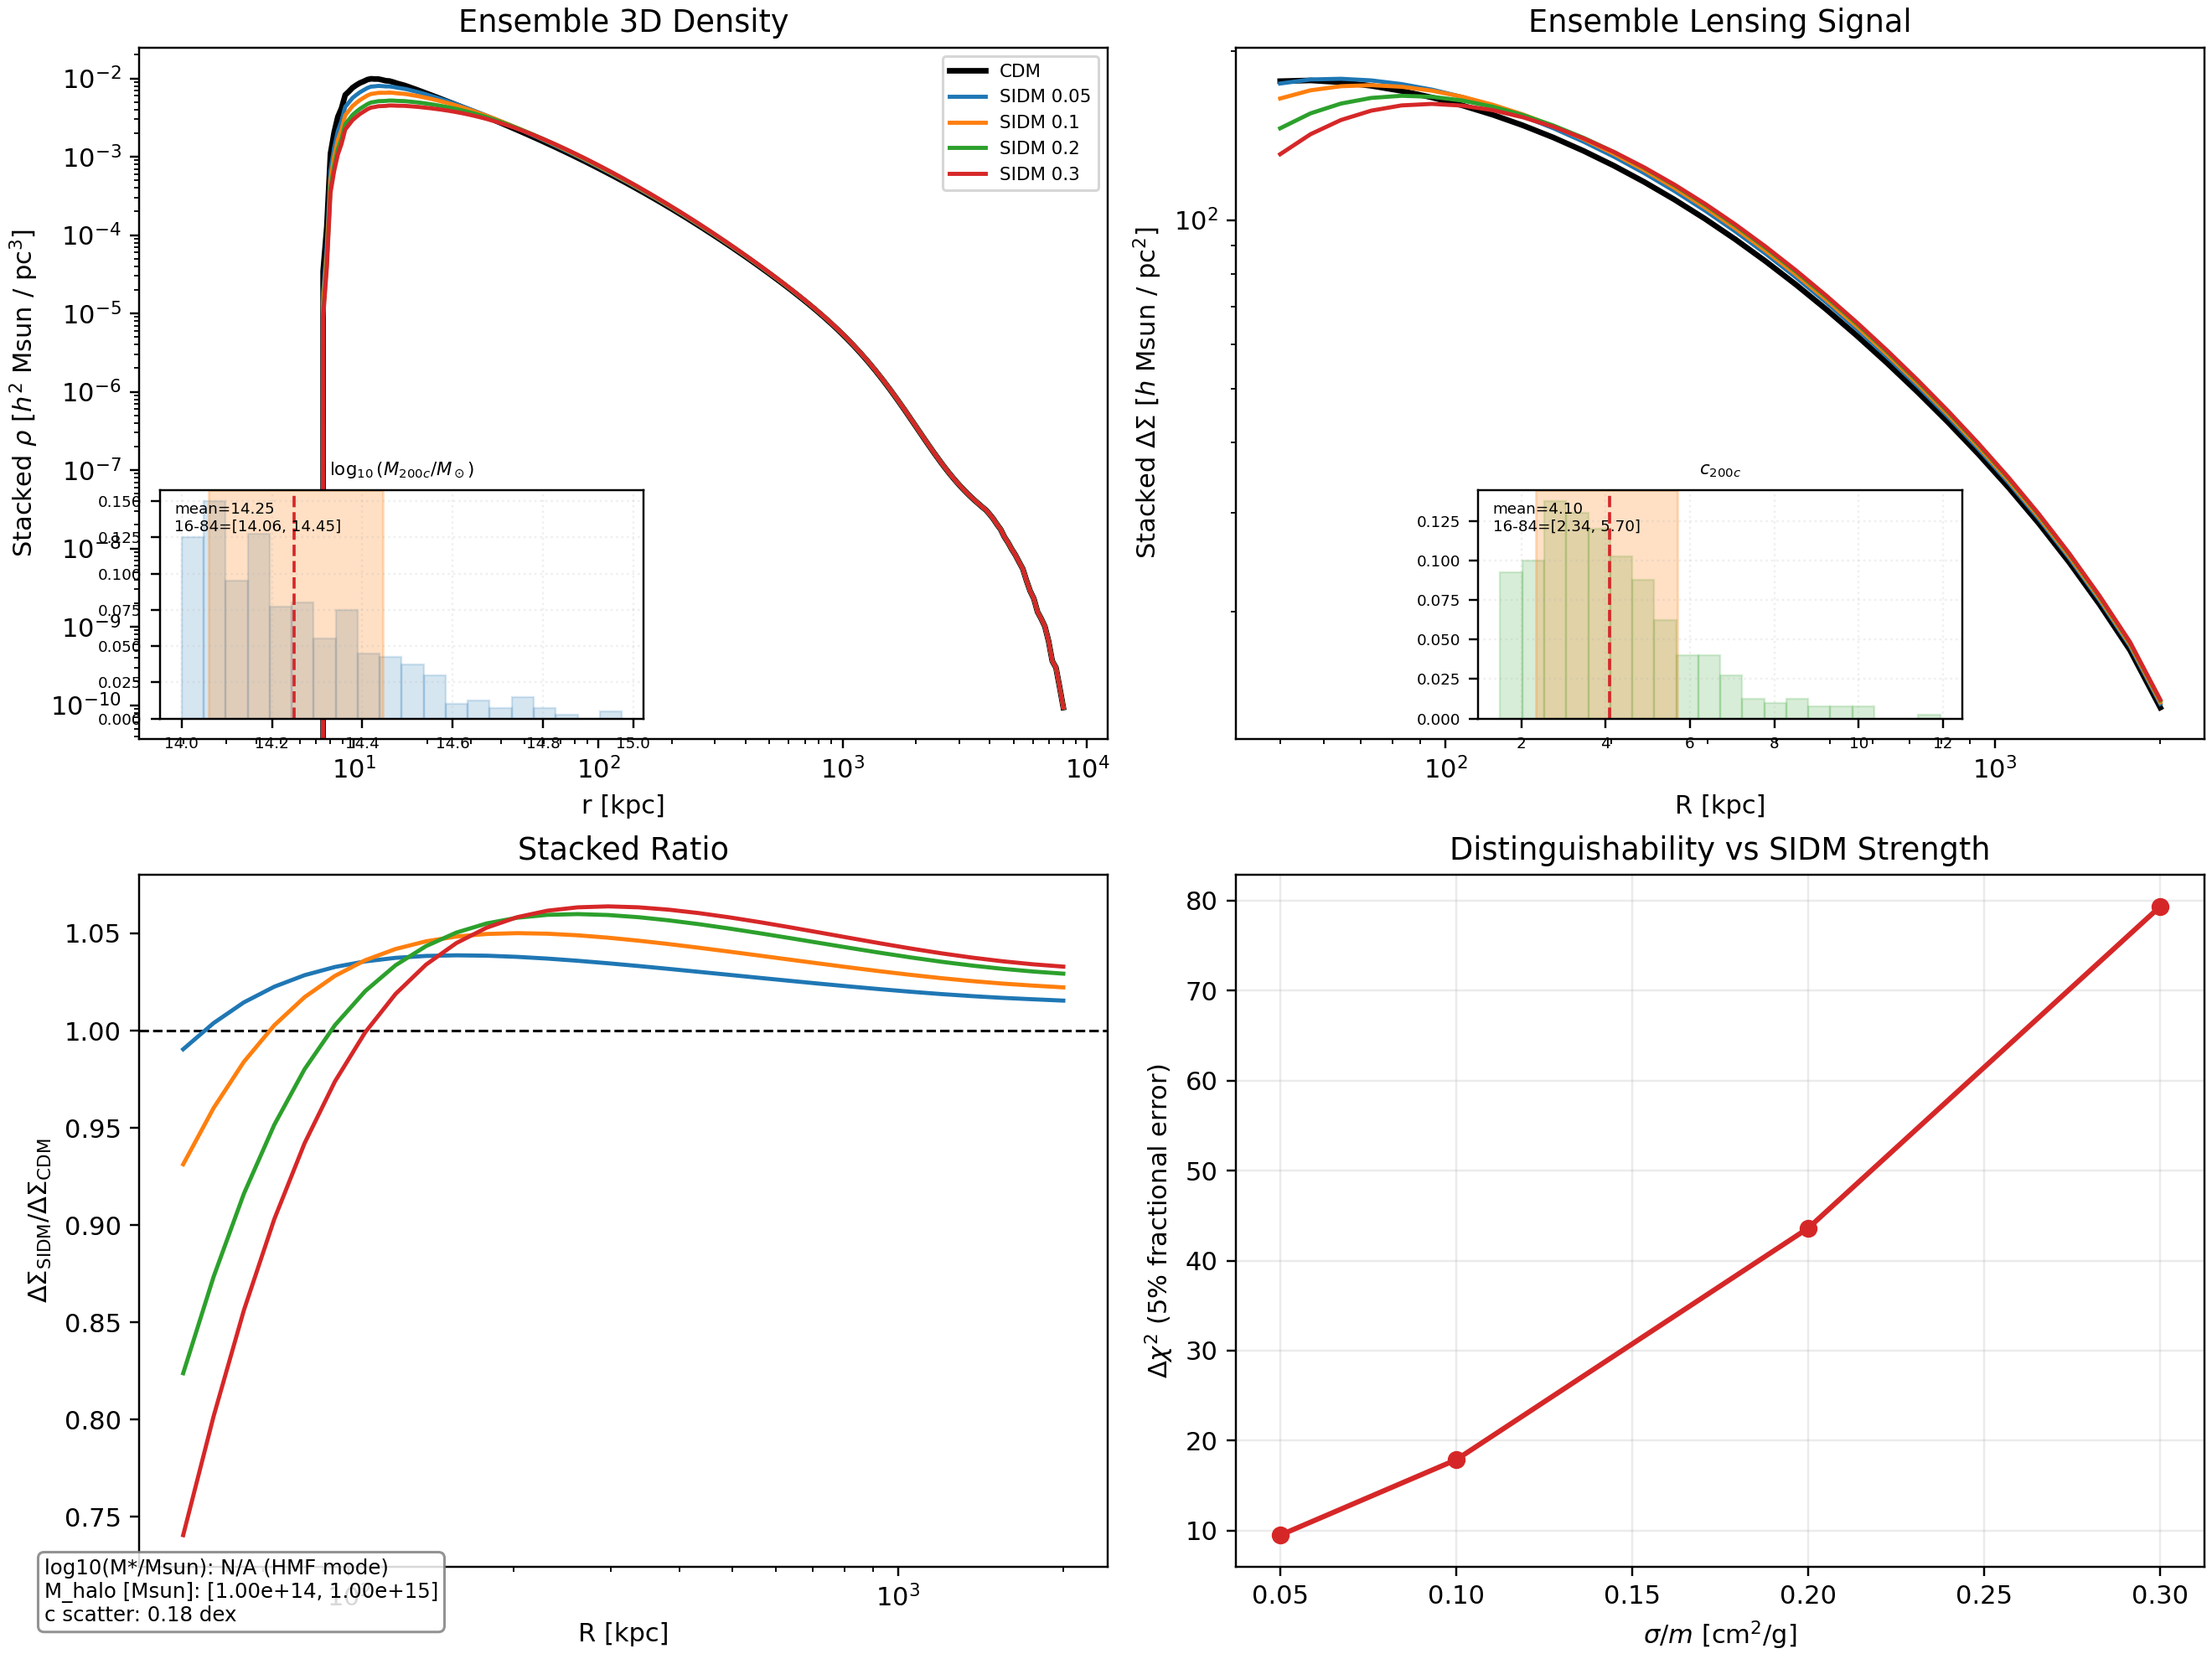
\includegraphics[width=0.92\textwidth]{figures/cluster_ensemble_summary.png}
    \caption{\textbf{Cluster ensemble summary (HMF-selected sample).} Multi-panel diagnostic from the current default cluster configuration (\texttt{docs/cluster\_ensemble\_config.yaml}), with Tier-2 hybrid profile treatment enabled. The figure summarizes stacked profile behavior over the benchmark sub-unity SIDM grid and reports toy $\Delta\chi^2$ sensitivity. As in the dwarf case, inset panels document the realized halo-mass and concentration distributions used in stacking. Interpretation caveat: cluster-side SIDM-like variations in $\Delta\Sigma$ can be degenerate with off-centering, concentration-selection effects, and baryonic profile modifications; these systematics are not yet jointly modeled in this first-order pipeline.}
    \label{fig:cluster_summary}
\end{figure}

\section{Findings and Caveats for White-Paper Use}
\textbf{Findings.}
\begin{itemize}[leftmargin=1.5em]
    \item The ensemble treatment is technically stable and reproducible (median-mass, radial-bin, fixed-seed, and single-halo-limit checks pass in the default cluster and dwarf runs).
    \item The stacked SIDM/CDM contrast is preserved after introducing realistic halo-population breadth, so the forecast is not an artifact of a single chosen halo.
    \item Tier-2 outer-profile attachment changes the large-radius baseline while retaining inner SIDM response, enabling more realistic cluster-scale profile comparisons.
\end{itemize}

\textbf{Caveats.}
\begin{itemize}[leftmargin=1.5em]
    \item The reported $\Delta\chi^2$ values are toy metrics tied to assumed fractional errors, not final survey-significance claims.
    \item Cluster interpretation is likely dominated by degeneracies with off-centering, concentration-population effects, and baryonic physics.
    \item No 2-halo term, full covariance, or full baryonic nuisance framework is included at this stage.
\end{itemize}

\appendix
\section{Appendix: Reproducibility Details}

\subsection{Configuration files}
\begin{itemize}[leftmargin=1.5em]
    \item Cluster baseline config: \texttt{docs/cluster\_ensemble\_config.yaml}
    \item Dwarf baseline config: \texttt{docs/dwarf\_ensemble\_config.yaml}
\end{itemize}

Key default settings:
\begin{itemize}[leftmargin=1.5em]
    \item Cluster: $N_{\mathrm{halos}}=400$, $M_{200c}\in[10^{14},10^{15}]\,M_\odot$, $z\sim\mathcal{N}(0.45,0.15)$ truncated to $[0.2,0.8]$, $\sigma_{\log c}=0.18$, $\sigma/m=\{0.05,0.1,0.2,0.3\}$ cm$^2$ g$^{-1}$.
    \item Dwarf: $N_{\mathrm{halos}}=800$, $\log_{10}M_\star\sim\mathcal{N}(7.5,0.5)$ truncated to $[6,9]$, SHMR scatter $0.3$ dex, $\sigma_{\log c}=0.20$, $\sigma/m=\{10,20,50,100\}$ cm$^2$ g$^{-1}$.
\end{itemize}

\subsection{Run commands}
\begin{verbatim}
python scripts/run_ensemble_forecast.py \
  --config-path docs/cluster_ensemble_config.yaml \
  --output-root outputs

python scripts/run_ensemble_forecast.py \
  --config-path docs/dwarf_ensemble_config.yaml \
  --output-root outputs
\end{verbatim}

\subsection{Primary outputs used in this note}
\begin{itemize}[leftmargin=1.5em]
    \item \texttt{outputs/figures/dwarf\_ensemble\_summary.png}
    \item \texttt{outputs/figures/cluster\_ensemble\_summary.png}
    \item \texttt{outputs/tables/dwarf\_ensemble\_delta\_chi2\_summary.csv}
    \item \texttt{outputs/tables/cluster\_ensemble\_delta\_chi2\_summary.csv}
    \item \texttt{outputs/tables/*\_ensemble\_validation\_checks.csv}
\end{itemize}

\subsection{Code modules}
\begin{itemize}[leftmargin=1.5em]
    \item Ensemble sampling: \texttt{src/sidm\_stagev\_forecast/ensemble.py}
    \item YAML normalization: \texttt{src/sidm\_stagev\_forecast/ensemble\_yaml.py}
    \item Profile construction: \texttt{src/sidm\_stagev\_forecast/profiles.py}
    \item Outer profile/stitching: \texttt{src/sidm\_stagev\_forecast/outer\_profiles.py}, \texttt{stitch.py}
    \item Projection: \texttt{src/sidm\_stagev\_forecast/projection.py}
    \item Stacking/forecast metrics: \texttt{src/sidm\_stagev\_forecast/stacking.py}, \texttt{forecast.py}
    \item Pipeline driver: \texttt{scripts/run\_ensemble\_forecast.py}
\end{itemize}

\end{document}
